\chapter{Manoeuvre loading diagrams}
\label{v-n_diagrams}
In this appendix the (V-n)-diagrams from all scenarios are shown. These scenarios were determined in \autoref{sec:Loading_Diagrams}


\begin{figure}[H]
    \centering
    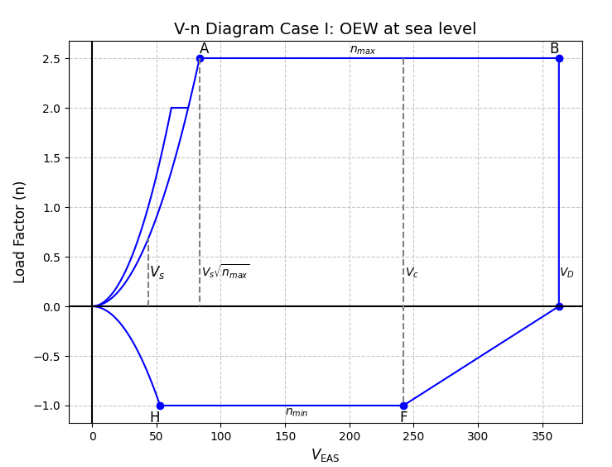
\includegraphics[width=0.65\linewidth]{figures/v-n diagram case I.png}
    \caption{V-n diagram for the aircraft operating at OEW at sea level}
    \label{fig:v-n_case1}
\end{figure}

\begin{figure}[H]
    \centering
    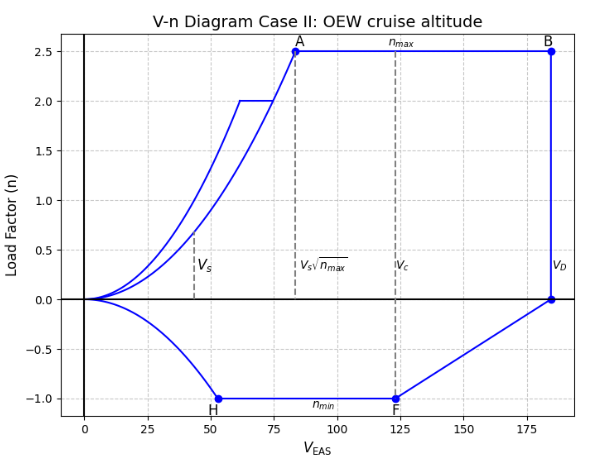
\includegraphics[width=0.65\linewidth]{figures/v-n diagram case II.png}
    \caption{V-n diagram for the aircraft operating at OEW at cruise altitude}
    \label{fig:v-n_case2}
\end{figure}

\begin{figure}[H]
    \centering
    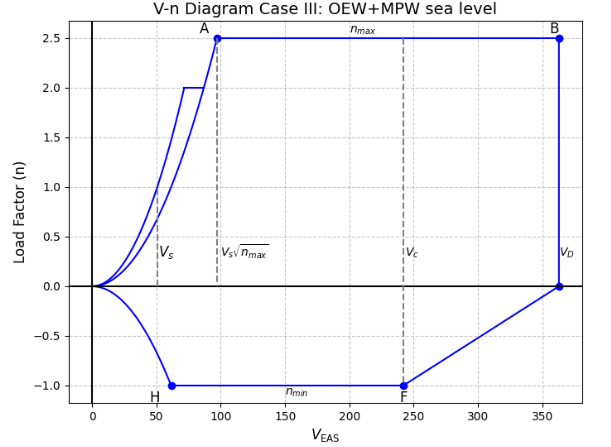
\includegraphics[width=0.65\linewidth]{figures/v-n diagram case III.png}
    \caption{V-n diagram for the aircraft operating at OEW and MPW at sea level}
    \label{fig:v-n_case3}
\end{figure}

\begin{figure}[H]
    \centering
    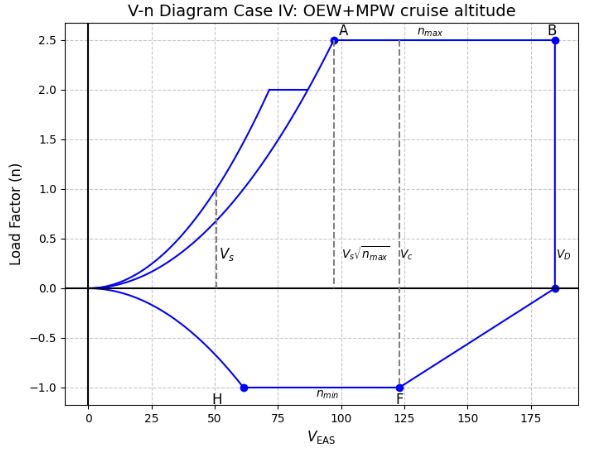
\includegraphics[width=0.65\linewidth]{figures/v-n diagram case IV.png}
    \caption{V-n diagram for the aircraft operating at OEW and MPW at cruise altitude}
    \label{fig:v-n_case4}
\end{figure}

\begin{figure}[H]
    \centering
    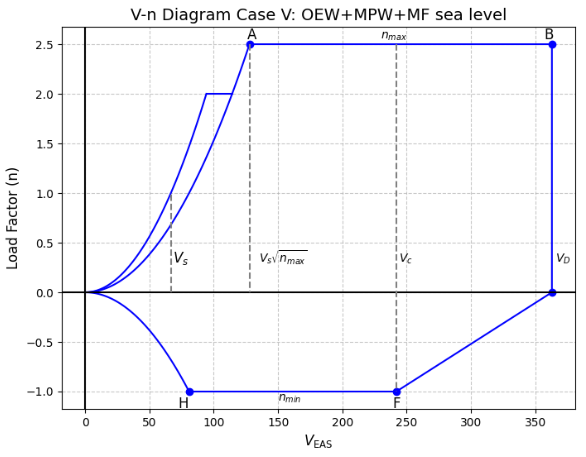
\includegraphics[width=0.65\linewidth]{figures/v-n diagram case V.png}
    \caption{V-n diagram for the aircraft operating at OEW, MPW and MF; at sea level conditions} 
    \label{fig:v-n_case5}
\end{figure}

\begin{figure}[H]
    \centering
    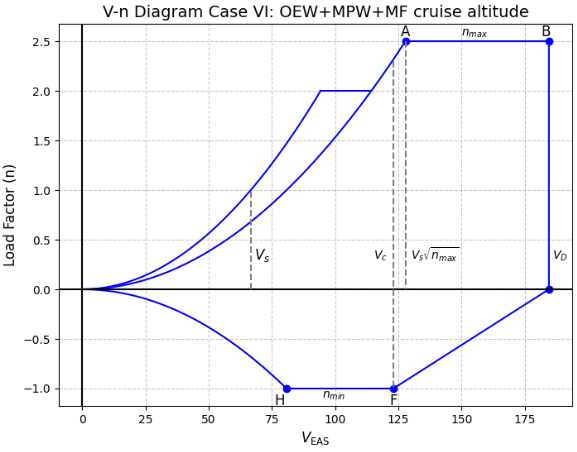
\includegraphics[width=0.65\linewidth]{figures/v-n diagram case VI.png}
    \caption{V-n diagram for the aircraft operating at OEW, MPW and MF; at cruise altitude}
    \label{fig:v-n_case6}
\end{figure}